
\section{Photon Identification}
\label{sec:photonID}
Photons from $\pi^0$ decays begin to merge into a single cluster in the EMCal above approximately  6~\GeVc. To identify clusters produced by single photons and reject clusters produced by two photons from a meson decay, we use variables that encode the shape of the calorimeter shower. %measured in the EMCal and DCal. We use the $\lambdasquare$ variable and a novel neural network variable; these are described in the next sections.

\subsection{Shower-shape variable}
The $\lambdasquare$ variable is the weighted root-mean-square of the shower energy along the major ellipse axis, defined according to~Ref.~\cite{Abelev:2014ffa} as:
\begin{equation}
\lambdasquare = \frac{s_{\eta\eta}+ s_{\phi\varphi}}{2} + \sqrt{   \frac{(s_{\eta\eta} - s_{\phi\varphi})^{2}}{4} + s^{2}_{\eta\varphi}         },
\end{equation}
where $s_{ij} = \langle ij \rangle - \langle i \rangle\langle j \rangle$ are the covariance matrix elements; the $i,j$ are cell indices in $\eta$ and  $\varphi$ axes; $\langle ij \rangle$ and $\langle i\rangle$, $\langle j\rangle$ are the second and the first moments of the cluster position cell weighted as follows:
\begin{equation}
\mathrm{weight} = \mathrm{max}\left(\log(E_{\mathrm{cell}}/E_{\mathrm{cluster}}), w_{0}\right). 
\end{equation}

Following previous work~\cite{Acharya:2018dqe}, we chose the cutoff in the log-weighting as $w_{0}=-4.5$, which means that cells that contain less than {$e^{-4.5} =$ 1.1$\%$} of the total cluster energy are not considered in the $\lambdasquare$ calculation.

Since $\lambdasquare$ represents the extent of the cluster, it discriminates between clusters belonging to single photons, for which the $\lambdasquare$ distribution is narrow and symmetric, and merged photons from neutral-meson decays, for which the distribution is dominated by a long tail towards higher values. 

%\subsection{Comparison of cluster distributions in pp and p-Pb data}
%Figure~\ref{fig:ppandpPbcomparison} shows a comparison between the transverse momentum and shower-shape distributions ($\lambdasquare$, DNN and $E_{\mathrm{max}}/E_{\mathrm{cluster}}$) in pp and p-Pb data for clusters that pass our selection. The distributions overlap to a large degree (at approximately the percent level), suggesting that the photon identification performance in both data taking periods is fairly similar even though they are separated by more than 4 years and the detector configurations are different (the DCal was installed in Run-2). This also severely constrains the degree of performance degradation due to higher underlying event density in p-Pb collisions. 

%\begin{figure}[h]
%\center
%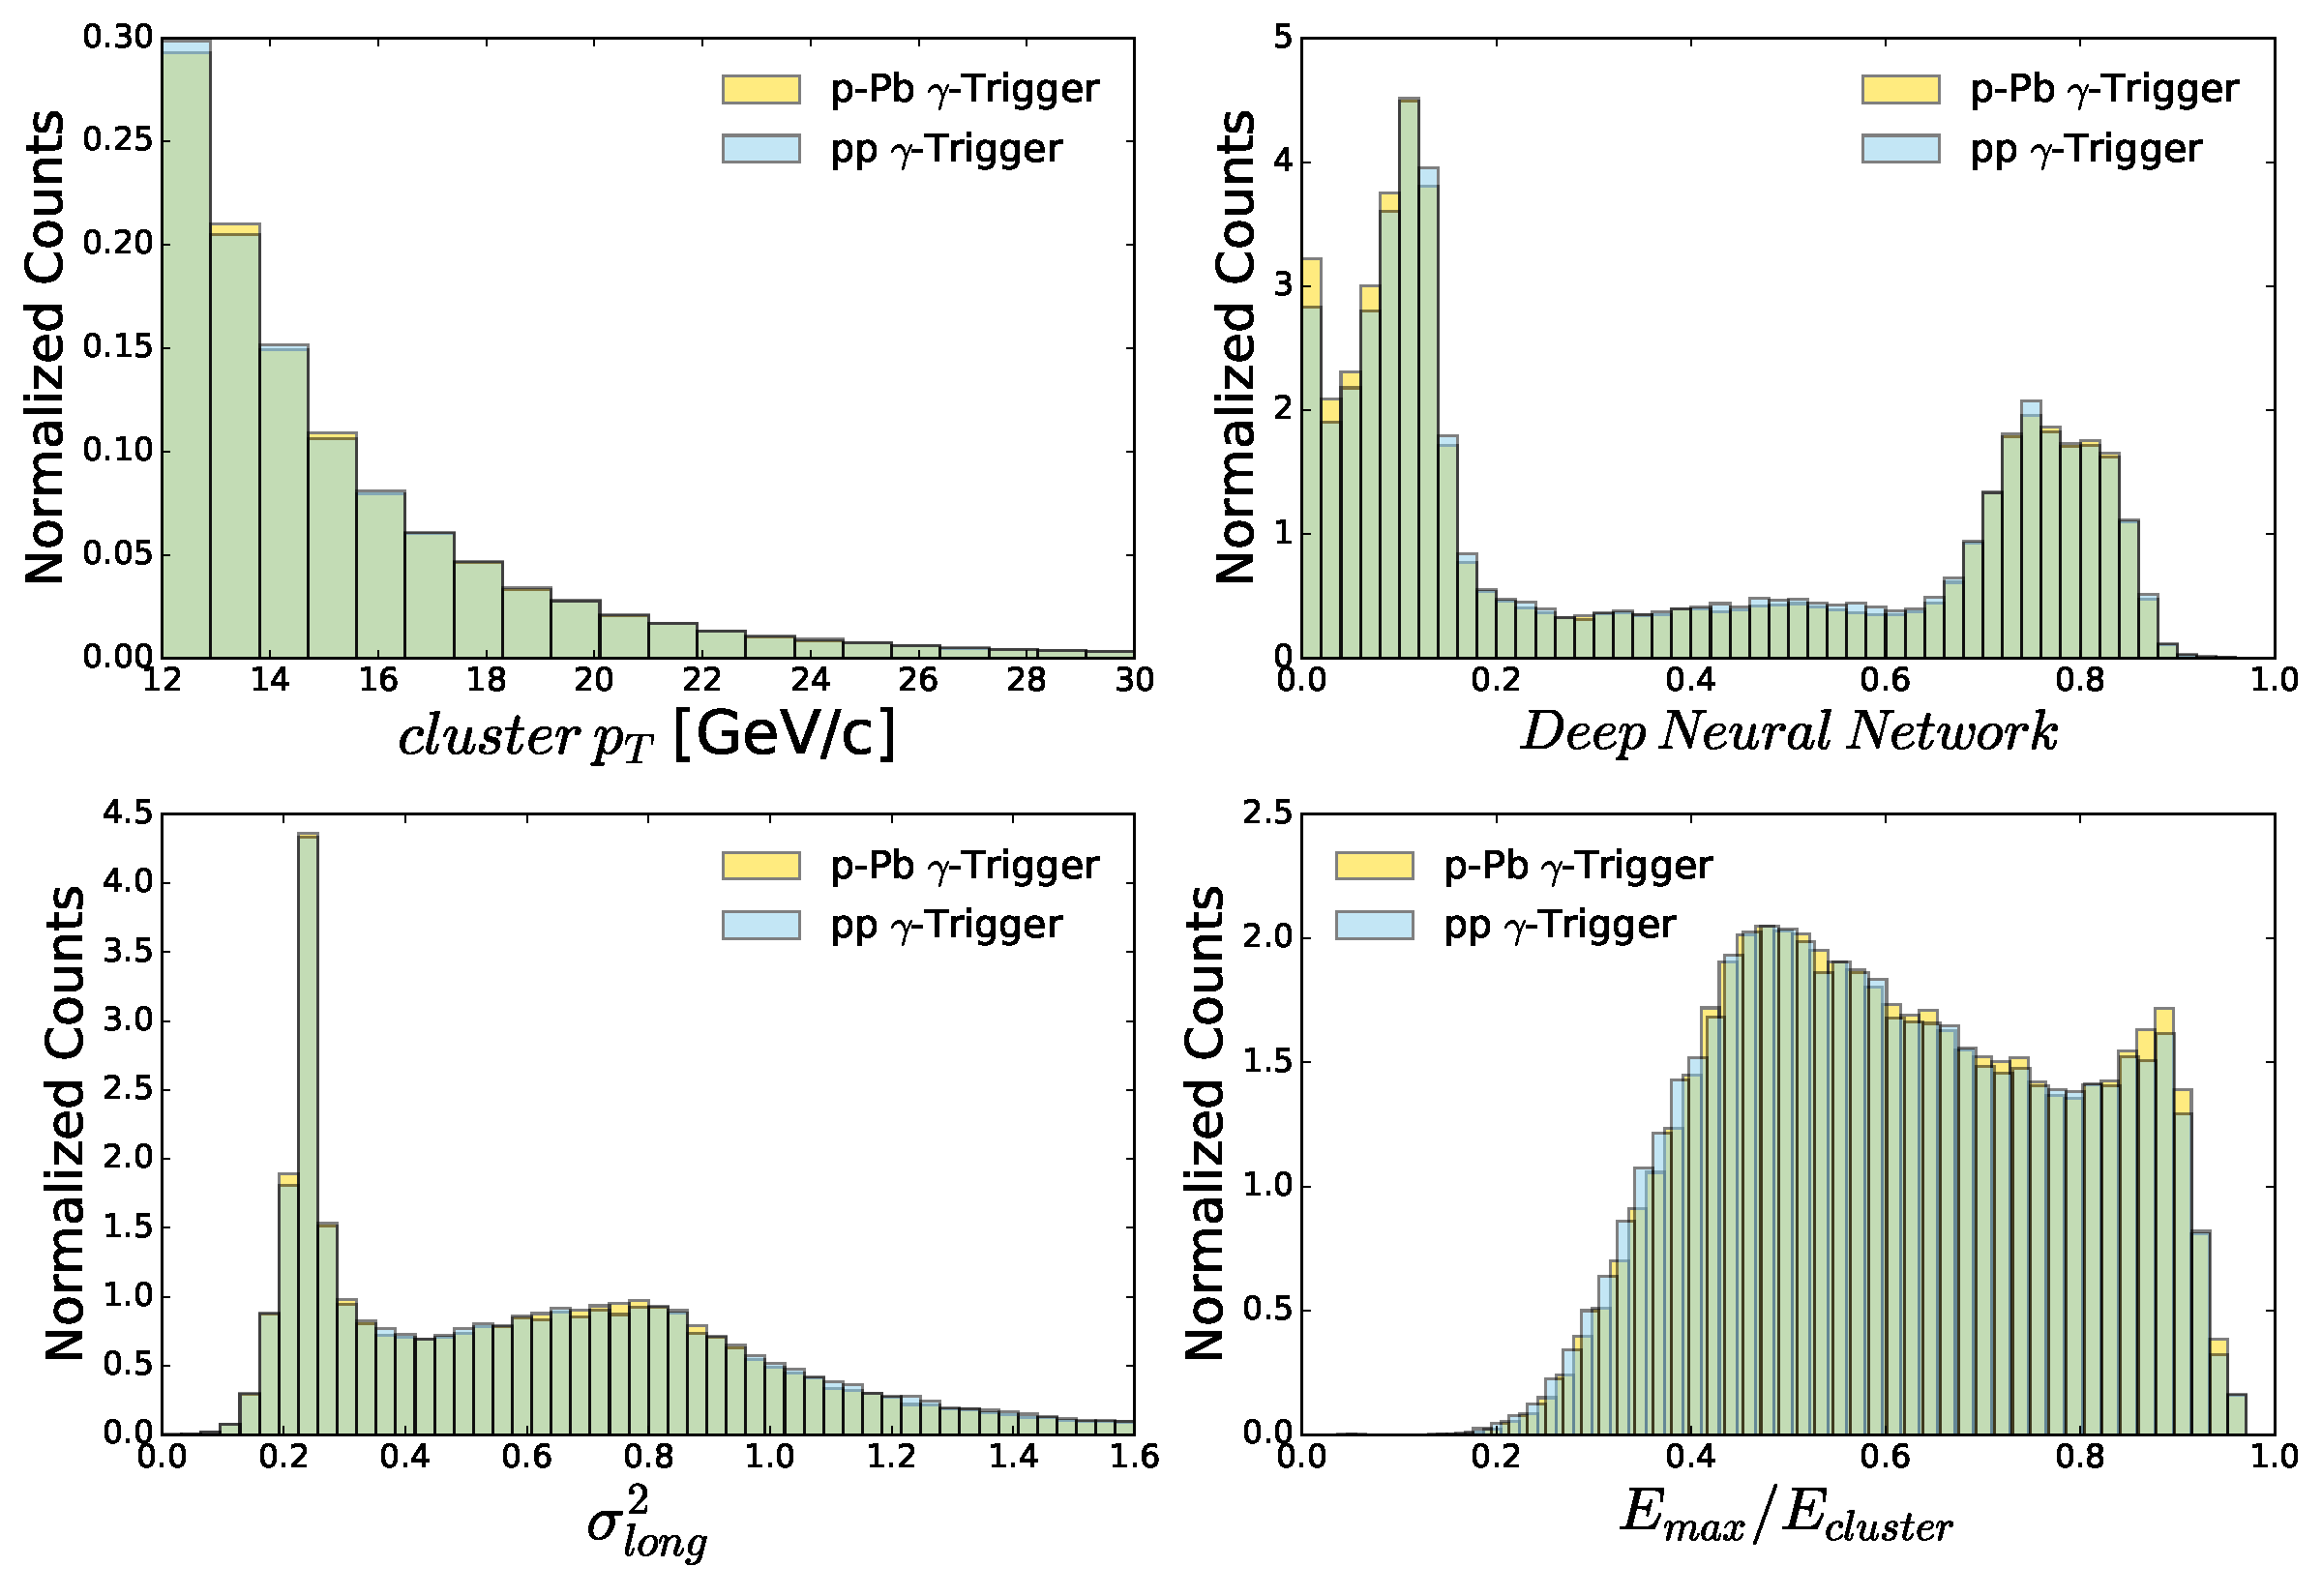
\includegraphics[width=0.9\textwidth]{EventAndClusterSelection/ppandpPbvariables.pdf}
%\caption{Transverse momentum and shower shape distributions for clusters that pass our selection in pp and p-Pb photon-triggered data. The overlap of the histograms is shown in green.}
%\label{fig:ppandpPbcomparison}
%\end{figure}

%\subsection{Comparison of cluster distributions in EMCal and DCal}
%Figure~\ref{fig:EMCALandDCALcomparison} shows a comparison between the transverse momentum and shower-shape distributions for clusters measured in EMCal and DCal in pp data. 
%\begin{figure}[h]
%\center
%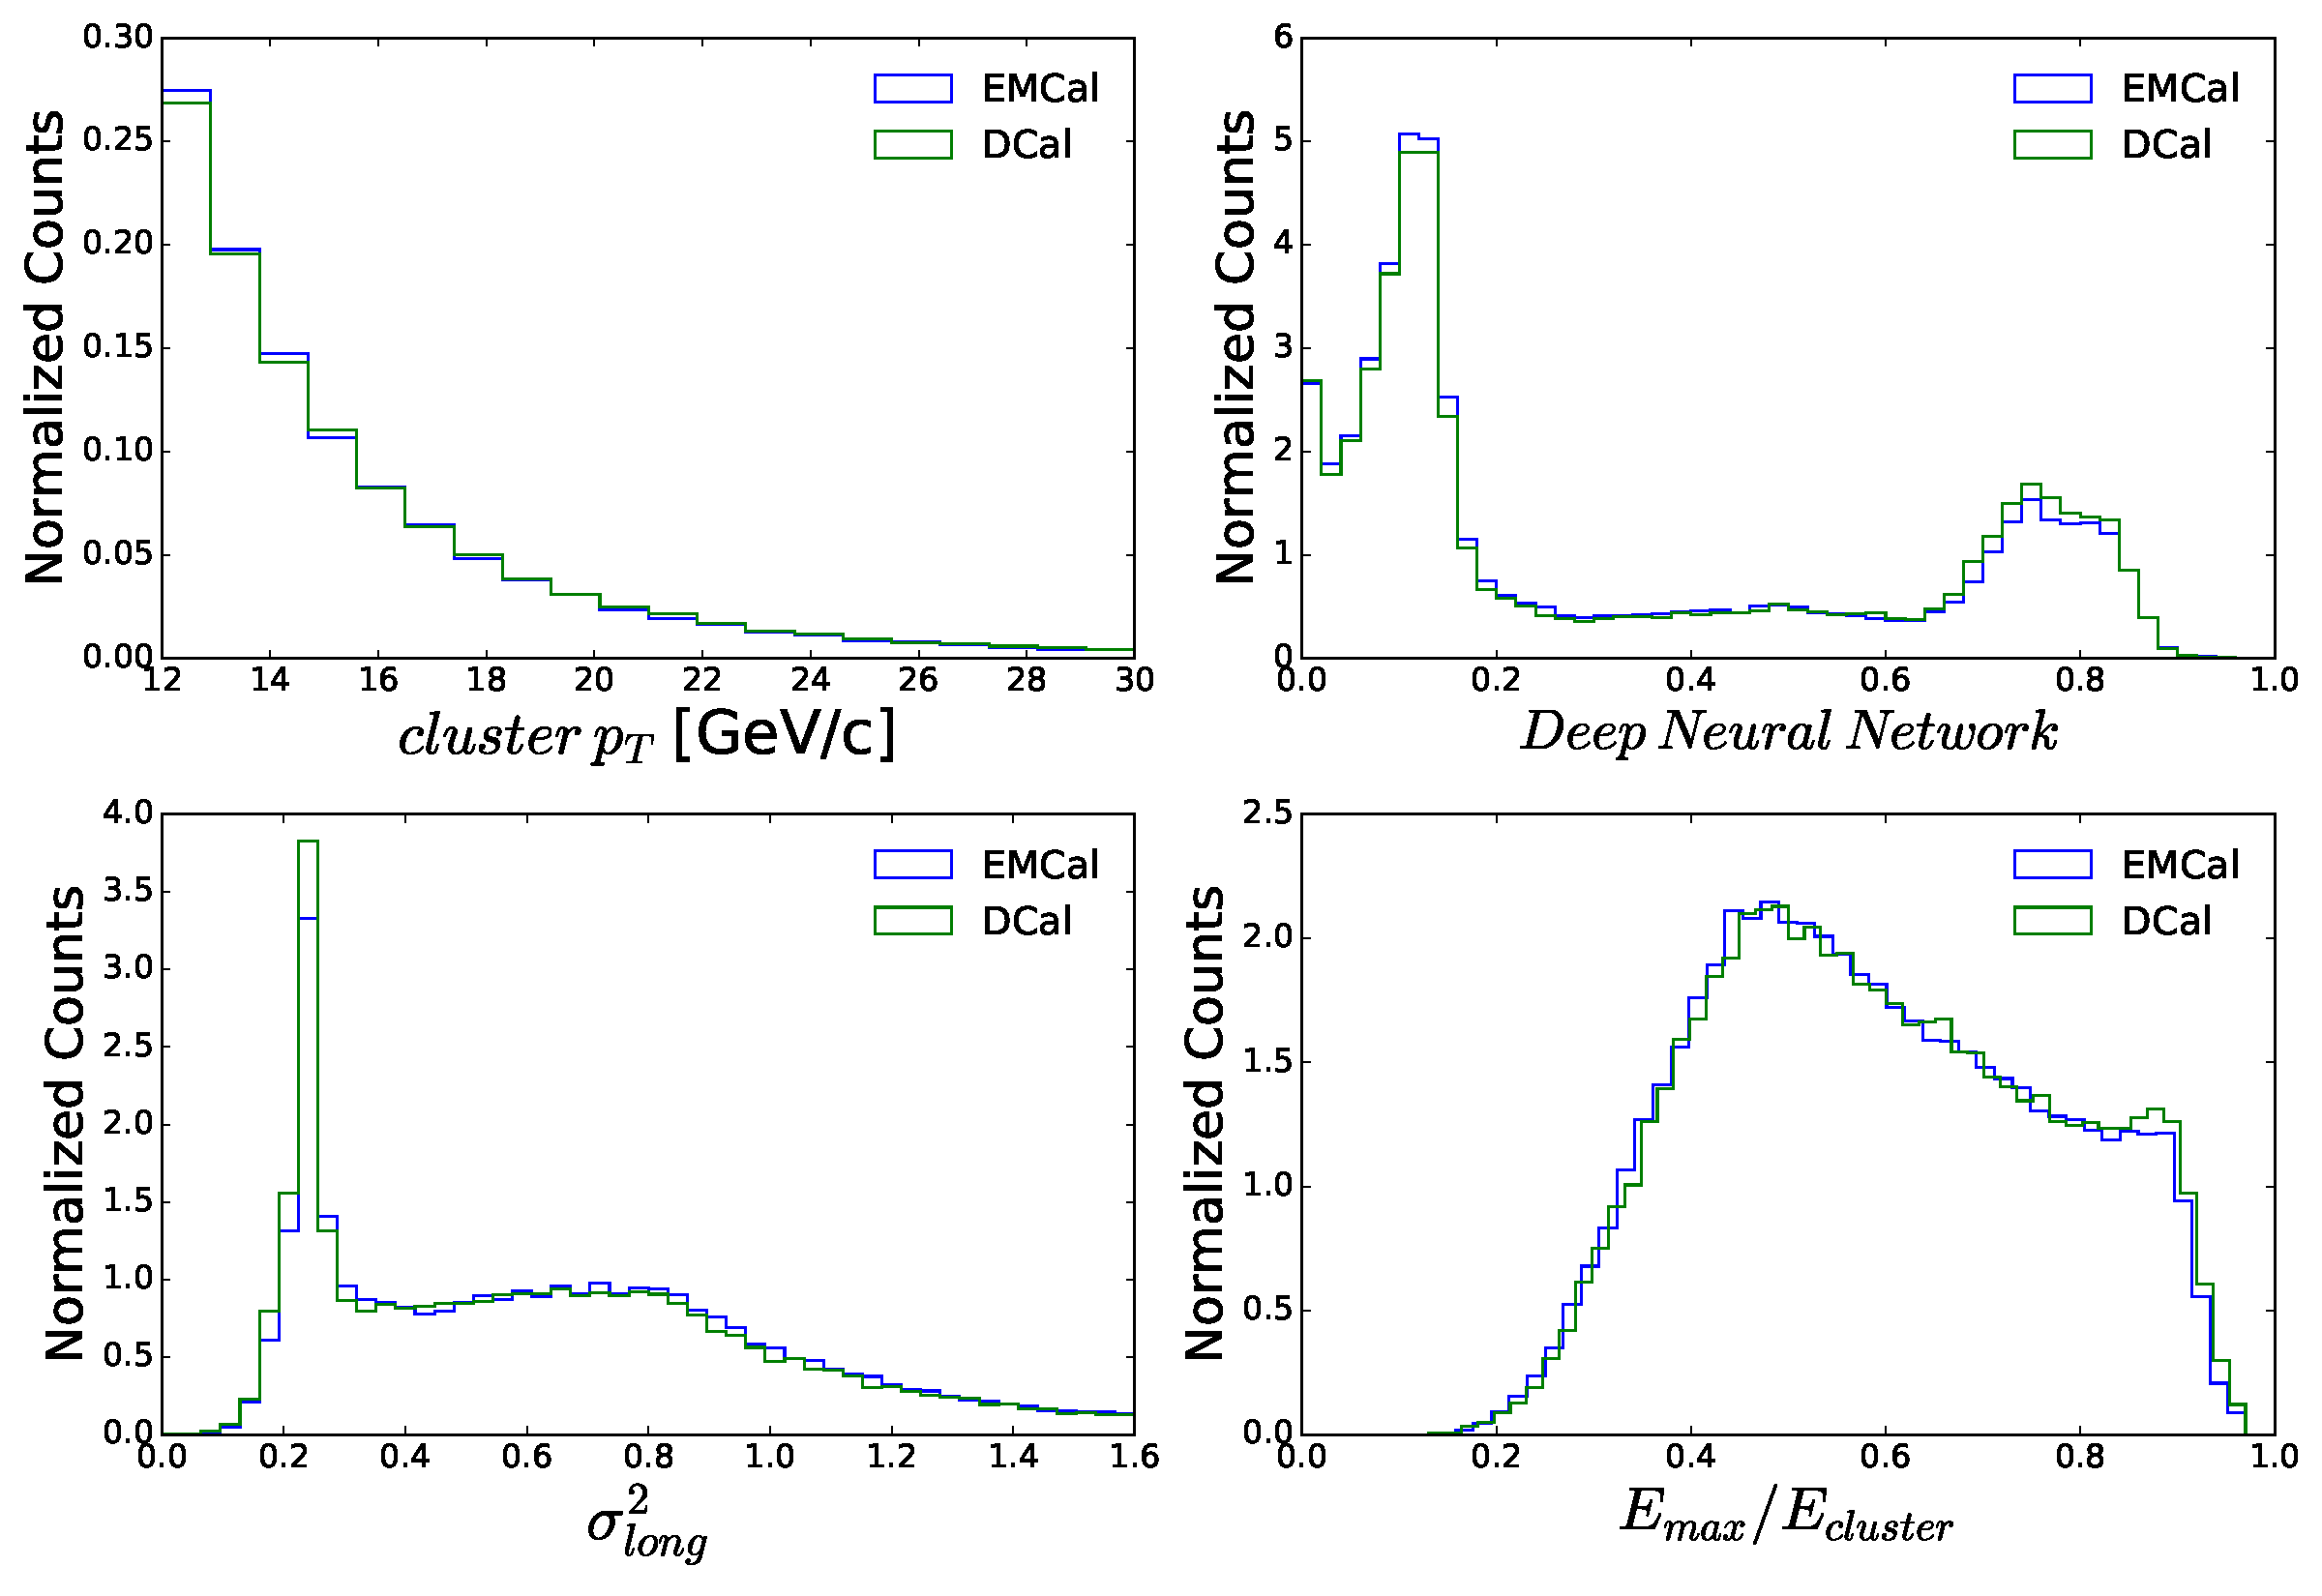
\includegraphics[width=0.9\textwidth]{EventAndClusterSelection/EMCAL_DCAL_variables.pdf}
%\caption{Transverse momentum and shower shape distributions for EMCal and DCal measured %clusters in pp photon-triggered data.}
%\label{fig:EMCALandDCALcomparison}
%\end{figure}

%The transverse momentum distributions are practically the same, which indicates that the EMCal and DCal absolute energy scales are very similar (otherwise a slope change would be expected). However, small but statistically significant differences in the shower-shape variables are observed. This is not surprising, given that is known that previous analyses have reported differences in the shower-shape measured for different super-modules. This is an effect that is attributed to cross-talk among the calorimeter cells, and is taken into account in the simulation, as shown in Section~\ref{sec:clusterselection}. 



%%%%%\subsection{Deep Neural Network}
%\label{sec:deepneuralnetwork}
%We have utilized a novel machine learning technique to improve the efficiency and purity of separating single and double photon clusters in the EMCal and DCal. Inspired by the similarities between pattern recognition in electromagnetic calorimeters and well-known image recognition problems, we utilize a deep neural network. The open-source neural network software package \textsc{TensorFlow} 1.7.0 was used~\cite{tensorflow2015-whitepaper}, first on a laptop, and then on the Cori supercomputer at NERSC~\cite{doi:10.1002/cpe.4291}.

%The neural network takes as input a $5\times 5$ array of the cells around each cluster's maximum cell. These 25 pieces of information, plus the cluster $\eta$, 1/$\sqrt{E_{\mathrm{cluster}}}$, the signed $\Delta\phi$ distance of the cluster to the closest supermodule center, and the V0M multiplicity, yield 29 parameters per cluster. We checked whether the neural network discrimination improves upon using a larger cell array, but found that 5x5 is sufficient. The $\eta$ and $\Delta\phi$ distance to the closest supermodule center are included to parametrize the residual nonprojectiveness, and possible alignment issues, while the V0M multiplicity enables the neural network weights to be applied across pp and p-Pb datasets (with possible extension to PbPb data).

%We utilized a neural network with 4 fully connected layers with 50 neurons each. After the 4th layer, 2 probabilistically motivated output neurons are formed from the output activations of the 4th layer, via the softmax function. One of these two neurons is tapped as the single photon discriminant.

%The neuron consists of the weight (a matrix multiplied with the input vector), a bias (the vector added after the matrix multiplication) and a suitable activation function. During the course of training, the each neuron learns an "activation", which is a real number usually close to $\pm 1$. Hence, a single neuron without the activation function is a linear classifier. The activation function -- termed analogously to the function of the firing rate in a biological neuron -- is needed to produce nonlinear classification.

%For this analysis, a Rectified Linear Unit (ReLU) activation function was used. It computes the function $f(x) = max(0,x)$, in effect setting a threshold for the activation at zero. Using a ReLU activation function greatly accelerates the convergence of stochastic gradient descent compared to the sigmoid or tanh functions. It has been argued that this is due to its linear, non-saturating form. However, a large gradient flowing through a ReLU neuron could cause the weights to update in such a way that the neuron will never activate on any datapoint again. If this happens, then the gradient flowing through the unit will forever be zero from that point on. That is, the ReLU units can irreversibly die during training. For example, as much as 40\% of a network can be ``dead'' (i.e. neurons that never activate across the entire training dataset) if the learning rate is set too high. This can be alleviated by making the network sufficiently large to allow for redundancy.

%After four layers, our neural network uses a binary softmax function to create a two-neuron output.  For example, one can interpret $\sigma(\sum_i w_ix_i+b)$
%to be the probability, P, of one of the final two neurons. The probability of the other final neuron would be 1 - P, since they must sum to one.

%The neural network was trained on photons from 8--30 GeV in simulated events, using an EM-enriched pPb Monte Carlo (ALICE LHC17g6a1, $\hat{p}_T$ bin 1--2, and LHC17g6a3, $\hat{p}_T$ bin 1--4, data sets), and 130K clusters each for training and test samples. Training was done using 128 batches and 12 epochs. The training time for each training sample was about 5 minutes on either a GPU or a Intel Knights Landing Xeon Phi.

%\subsection{Verification of DNN in LHC16k (13 TeV pp)}

%In order to confirm that the DNN is truly selecting on single photons, the $\eta \rightarrow \gamma\gamma$ channel in the intermediate ($\approx 10\:\mathrm{GeV}$) can be used to identify prompt single photons. The $\eta$ is optimum for this due to the larger opening angles, so the two decay photons are not merged until higher $p_T$. However, due to the statistics limitation in lower $\sqrt{s}$ (collision systems taken with LHC HI budget), the 13 TeV pp is preferable. We utilize data from LHC16k, which is the largest, triggered run period in 2016.

%For the LHC16k study, the following DPG runs with good TPC and EMCAL performance are selected:
%\begin{quote}
%258537, 258499, 258477, 258456, 258454, 258426, 258393, 258387, 258359, 258336, 258299, 258278, 258274, 258273, 258271, 258270, 258258, 258257, 258256, 258204, 258203, 258202, 258198, 258197, 258178, 258117, 258114, 258113, 258109, 258108, 258107, 258063, 258062, 258059, 258049, 258048, 258045, 258042, 258019, 258017, 258014, 258012, 257963, 257960, 257958, 257957, 257939, 257937, 257936, 257893, 257892, 257855, 257850, 257803, 257800, 257799, 257798, 257797, 257773, 257765, 257754, 257737, 257735, 257734, 257733, 257724, 257697, 257694, 257692, 257691, 257689, 257687, 257682, 257642, 257606, 257605, 257594, 257590, 257587, 257566, 257562, 257561, 257560, 257541, 257540, 257539, 257537, 257531, 257530, 257492, 257491, 257490, 257487, 257474, 257457, 257320, 257260, 257224, 257209, 257206, 257204, 257145, 257144, 257142, 257141, 257140, 257139, 257138, 257137, 257136, 257100, 257092, 257084, 257083, 257082, 257080, 257077, 257026, 257021, 257012, 257011, 256944, 256942, 256941, 256697, 256695, 256694, 256692, 256691, 256684, 256681, 256677, 256676, 256658, 256620, 256619, 256592, 256591, 256589, 256567, 256565, 256564, 256562, 256561, 256560, 256556, 256554, 256552, 256514, 256512, 256510, 256506, 256504
%\end{quote}
%The reconstruction used is pass1.

%For the MC comparison, the LO $\gamma$-jet (since this is where the signal template originates) LHC17i3a1 sample is used, where the first 4 $\hat{p}_T$ are used, and cross section/``ntrials'' merged. The run list consists of the intersection of LHC17i3a1 with the DPG validated LHC16k runs, namely:
%\begin{quote}
%256504, 256506, 256510, 256512, 256554, 256556, 256560, 256561, 256562, 256564, 256565, 256567, 256589, 256591, 256592, 256619, 256620, 256658, 256676, 256677, 256681, 256684, 256691, 256692, 256694, 256695, 256697, 256942, 256944, 257011, 257021, 257077, 257080, 257082, 257084, 257092, 257100, 257136, 257138, 257139, 257140, 257141, 257142, 257144, 257145, 257204, 257206, 257209, 257260, 257474, 257487, 257490, 257491, 257492, 257530, 257531, 257540, 257541, 257560, 257561, 257562, 257566, 257587, 257590, 257605, 257606, 257642, 257682, 257687, 257689, 257697, 257724, 257733, 257735, 257737, 257754, 257765, 257773, 257797, 257798, 257799, 257800, 257803, 257850, 257892, 257893, 257936, 257937, 257939, 257957, 257958, 257960, 258012
%\end{quote}

%Even though it is possible to perform a comparison with the LO photon in the $\gamma$-jet sample, the only origin for track MIP contamination on the LO photon side is initial and final state radiation; thus the contamination will be unrealistically low. For this reason, the same selection to reconstruct $\eta$ is applied also to MC, with the downside that the statistics will be limited.

%Because LHC16k contains pile-up events, for event selection in the data, any event containing a 2nd SPD vertex is vetoed.

%The following standard cluster selection are applied to both data and MC:
%\begin{equation}
%\begin{split}
%N_\mathrm{cell} &\ge 2\\
%0.1 &< \lambdasquare < 0.7\\
%E_\mathrm{cross} &< 0.05 E_\mathrm{max}\\
%\end{split}
%\end{equation}
%To maximally remove MIP contamination, clusters with any tracks within 3 cell distance on the surface of the EMCAL is vetoed. Finally, in order to enhance the diphoton signal, the asymmetry cut
%\begin{equation}
%\left\lvert\frac{E_1 - E_2}{E_1 + E_2}\right\rvert < 0.5
%\end{equation}
%is applied.

%The diphoton mass is split into a signal region with $0.5 < m_{\gamma\gamma} < 0.6\:\mathrm{GeV}/c^2$, and two background regions with $0.325 < m_{\gamma\gamma} < 0.475\:\mathrm{GeV}/c^2$ and $0.625 < m_{\gamma\gamma} < 0.775\:\mathrm{GeV}/c^2$. Because the background appears approximately linear, the signal and background are simply integrated (with the symmetric choice as stated), then normalized by unit $m_{\gamma\gamma}$, and the background distribution subtracted from the signal distribution.

%\begin{figure}[th]
%\centerline{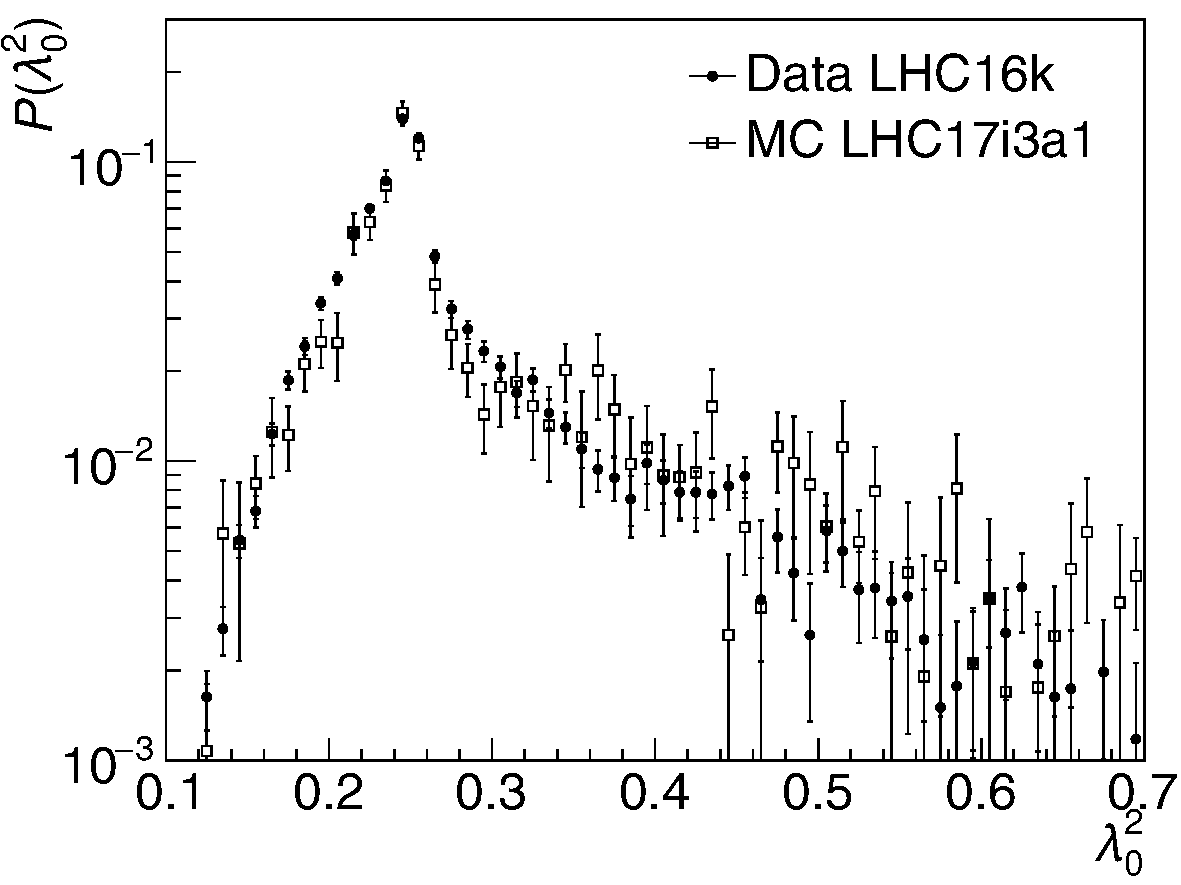
\includegraphics[width=0.3333\textwidth]{eta_lambda02_08_12}%
%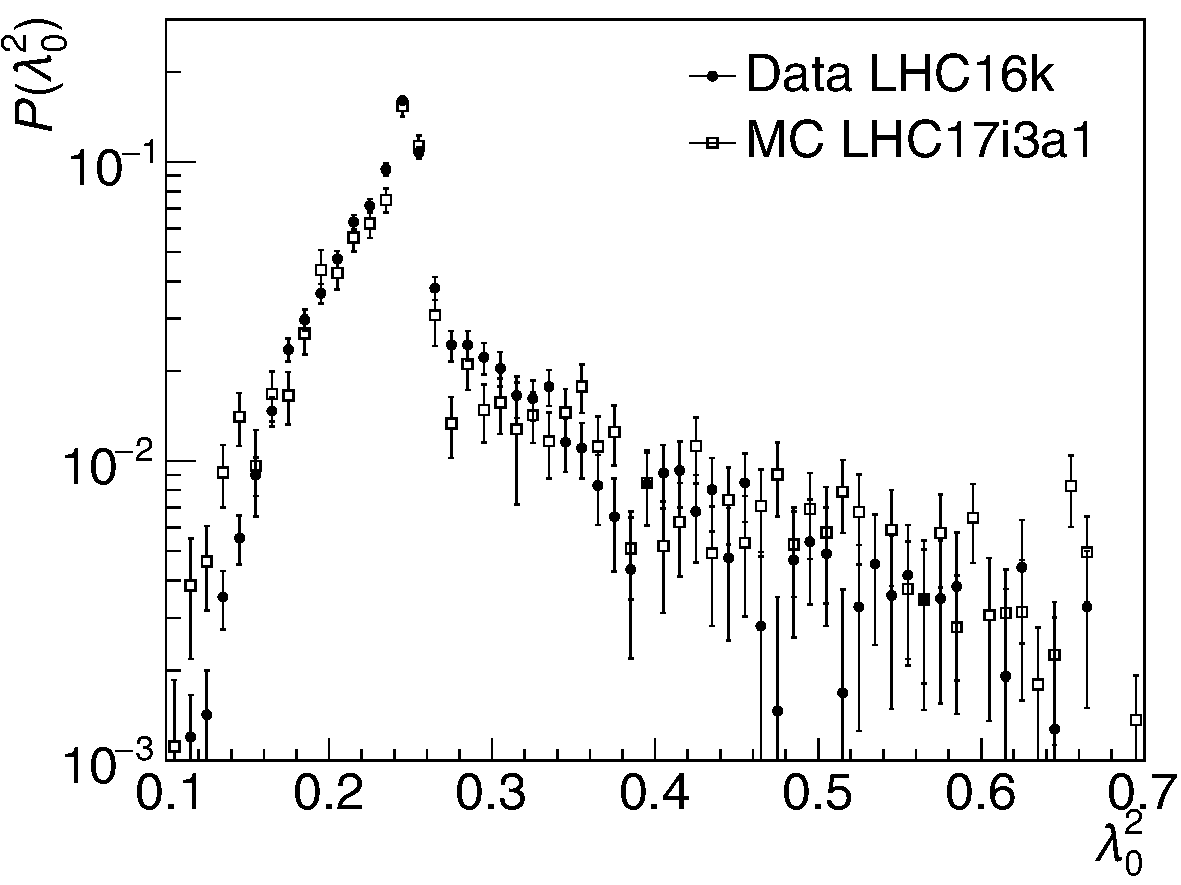
\includegraphics[width=0.3333\textwidth]{eta_lambda02_12_20}%
%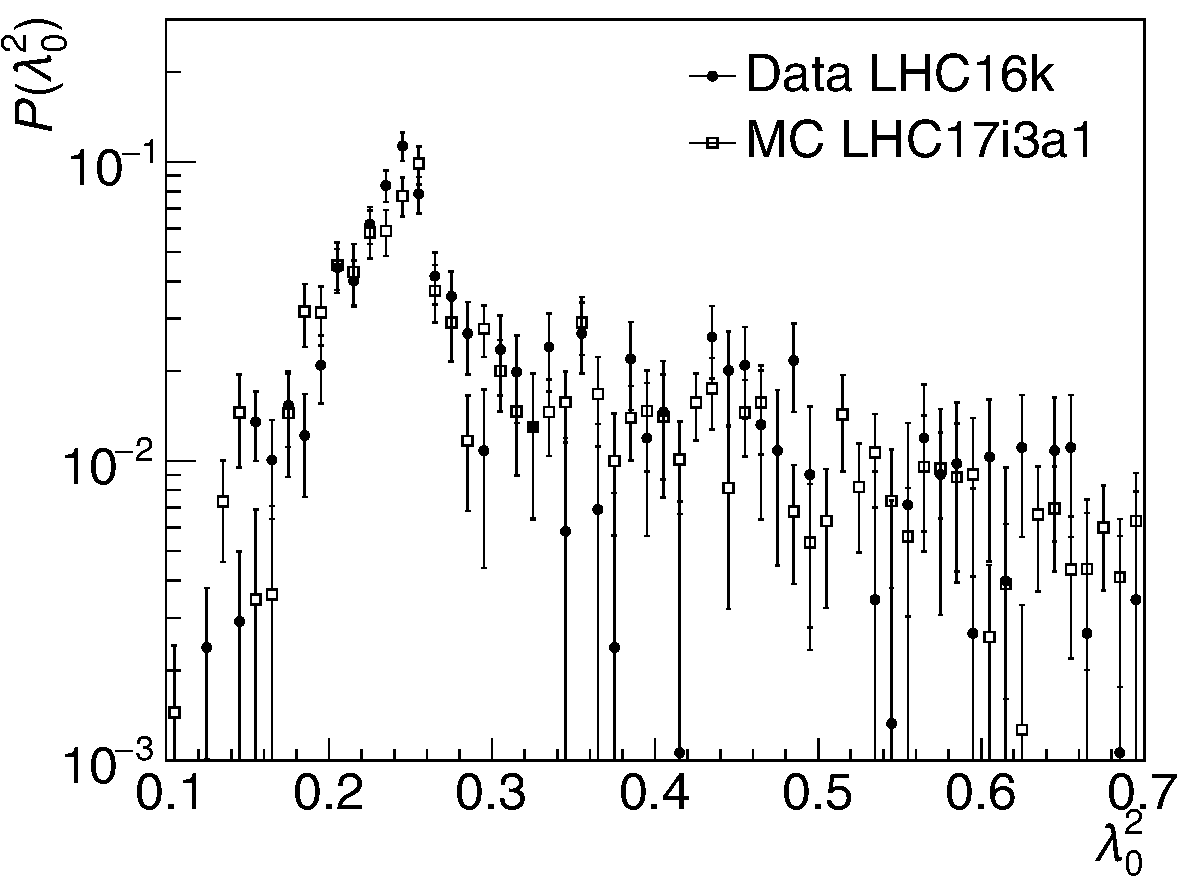
\includegraphics[width=0.3333\textwidth]{eta_lambda02_20_30}}
%\centerline{\hfill$8 \le E_\gamma < 12\:\mathrm{GeV}$\hfill\hfill$12 \le E_\gamma < 20\:\mathrm{GeV}$\hfill\hfill$20 \le E_\gamma < 30\:\mathrm{GeV}$\hfill}
%\centerline{\hfill$\chi^2/\text{DOF} = 1.21$\hfill\hfill$\chi^2/\text{DOF} = 1.82$\hfill\hfill$\chi^2/\text{DOF} = 1.48$\hfill}
%\caption{The distribution of $\lambdasquare$ for single photons, using $\eta \rightarrow \gamma\gamma$, comparing LHC16k with LHC17i3a1 MC. Because the shape only subtlely depend on single vs. two photons, the $E_\gamma$ dependence is weak.}
%\label{fig:eta_lambda02}
%\end{figure}

%\begin{figure}[th]
%\centerline{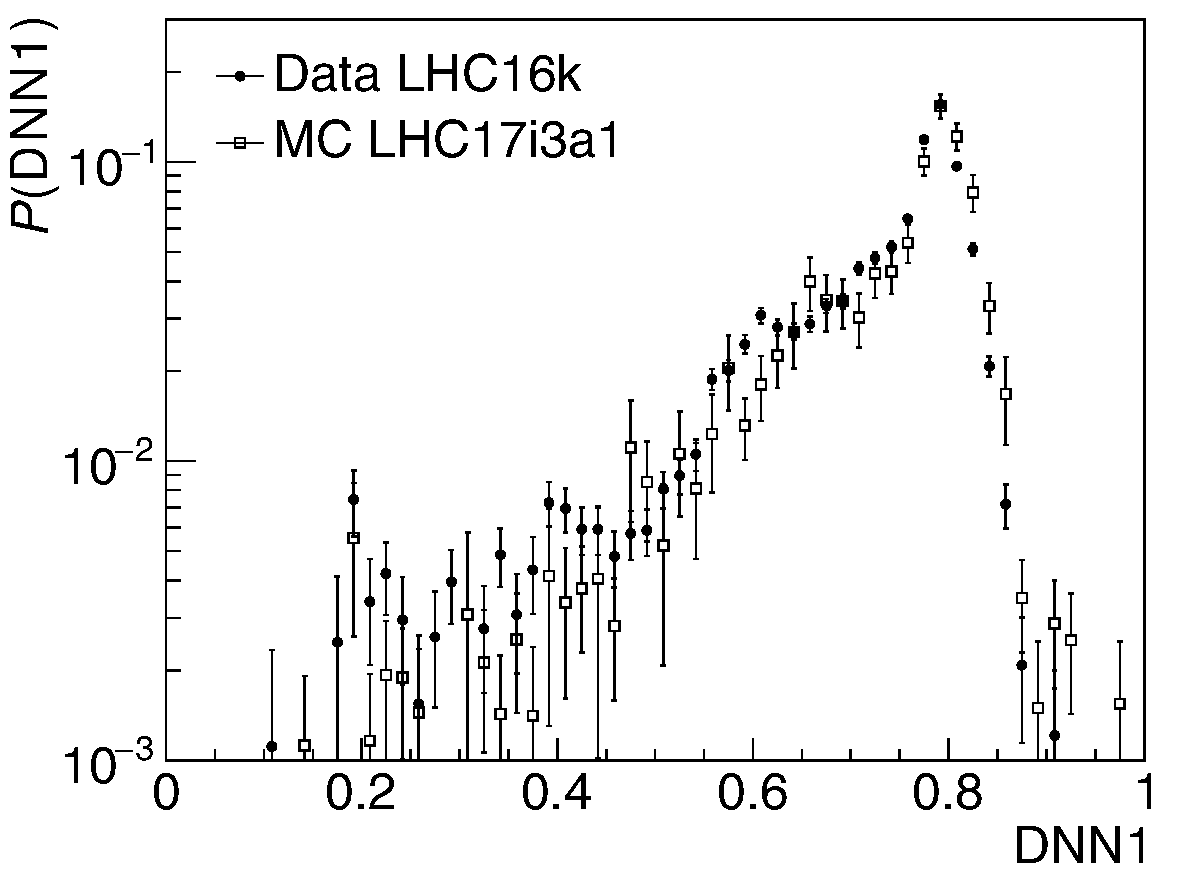
\includegraphics[width=0.3333\textwidth]{eta_dnn_08_12}%
%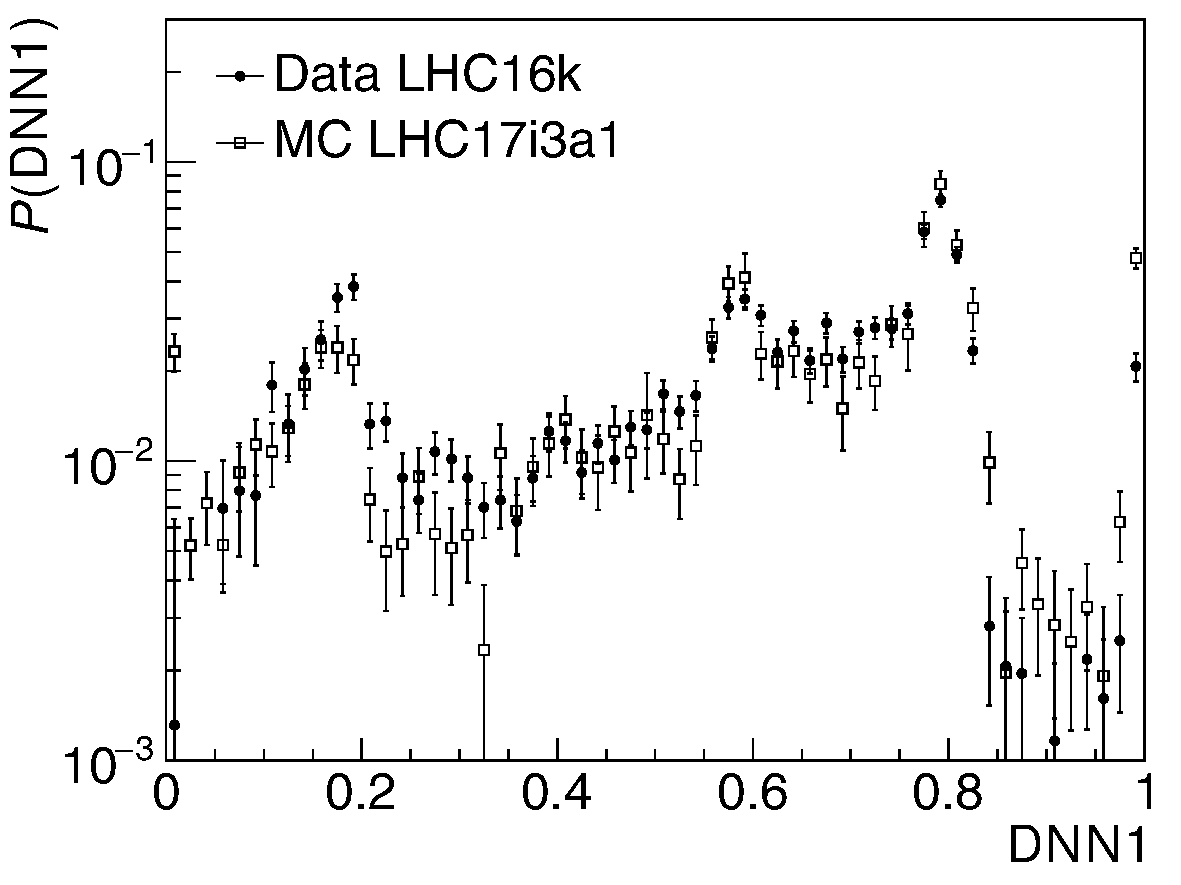
\includegraphics[width=0.3333\textwidth]{eta_dnn_12_20}%
%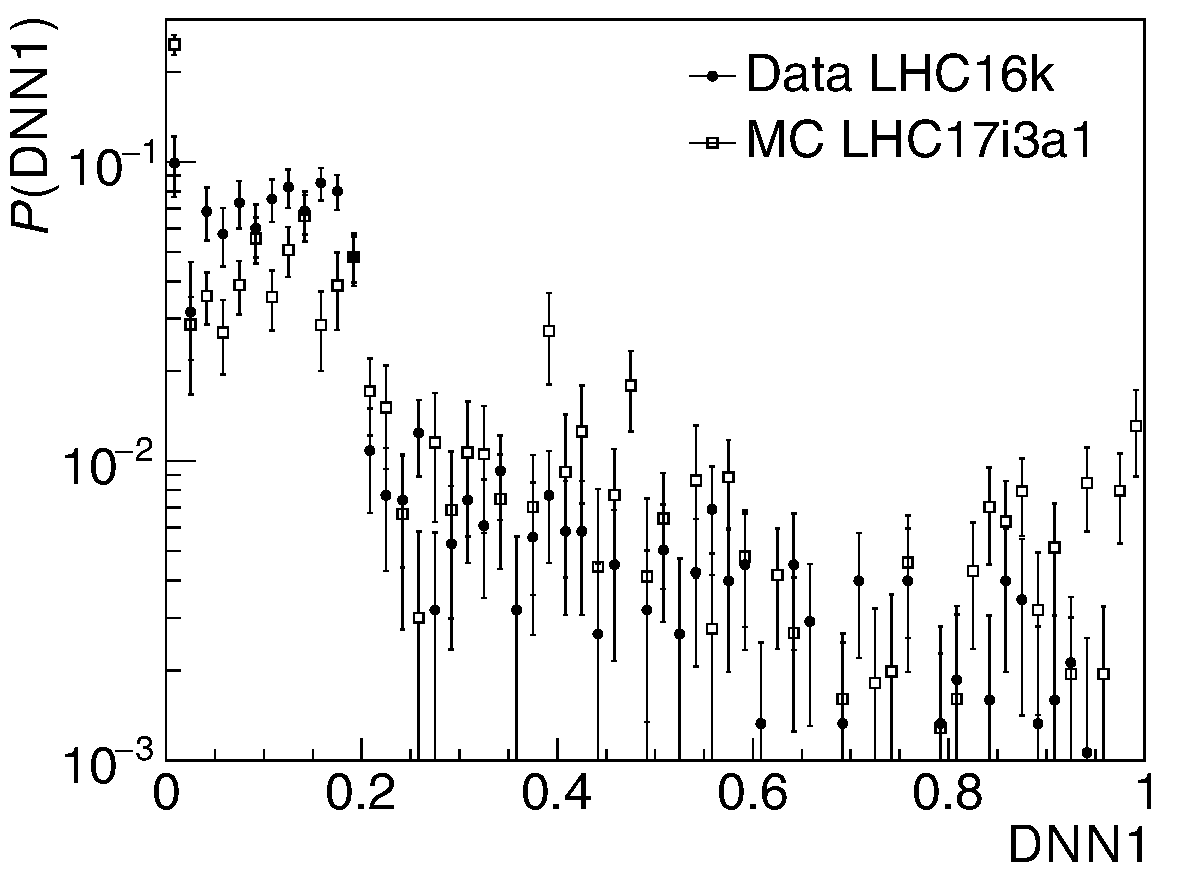
\includegraphics[width=0.3333\textwidth]{eta_dnn_20_30}}
%\centerline{\hfill$8 \le E_\gamma < 12\:\mathrm{GeV}$\hfill\hfill$12 \le E_\gamma < 20\:\mathrm{GeV}$\hfill\hfill$20 \le E_\gamma < 30\:\mathrm{GeV}$\hfill}
%\centerline{\hfill$\chi^2/\text{DOF} = 3.00$\hfill\hfill$\chi^2/\text{DOF} = 2.82$\hfill\hfill$\chi^2/\text{DOF} = 2.68 $\hfill}
%\caption{DNN activation for single photons, using $\eta \rightarrow \gamma\gamma$, comparing LHC16k with LHC17i3a1 MC. Note that for progressively higher energy photons, cluster merging occurs, and the activation starts to resemble $\pi^0 \rightarrow \gamma\gamma$ at lower energies.}
%\label{fig:eta_dnn}
%\end{figure}

%\begin{figure}[th]
%\centerline{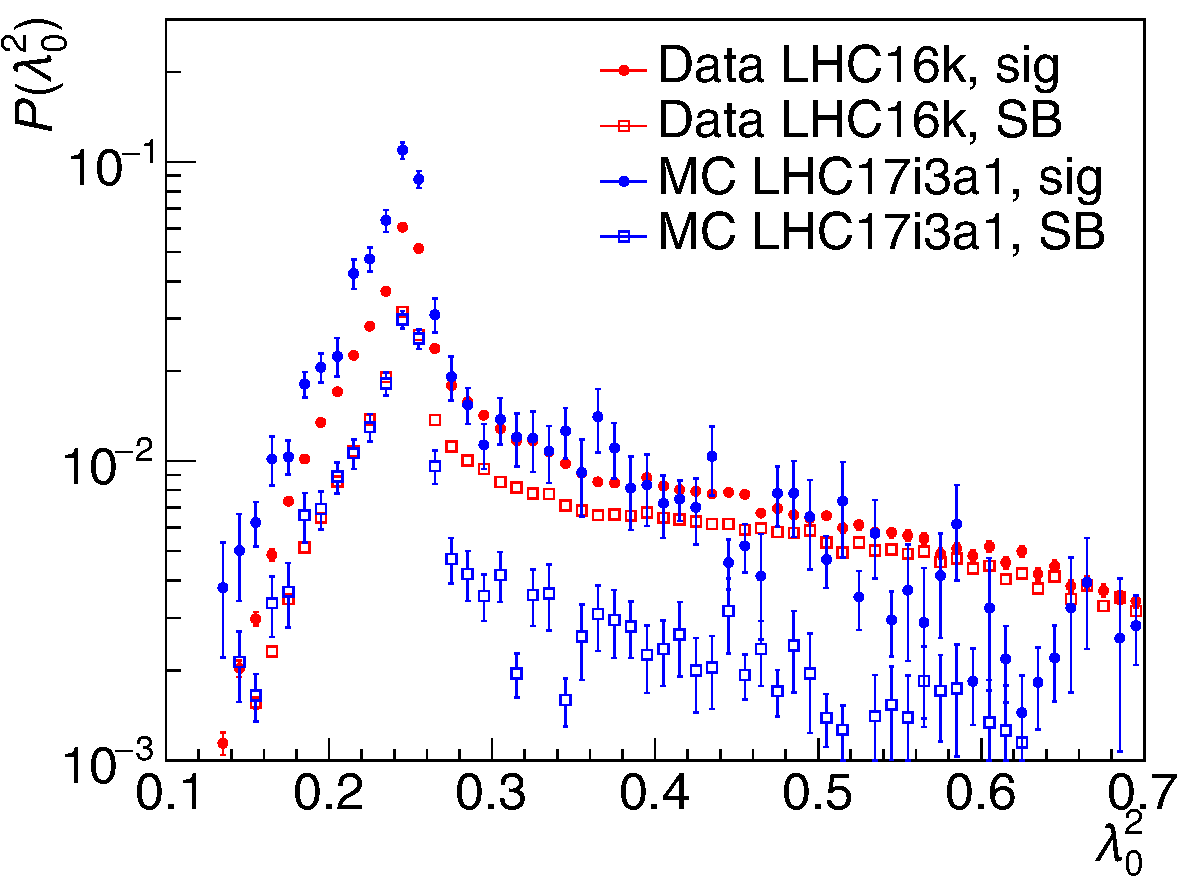
\includegraphics[width=0.5\textwidth]{eta_lambda02_08_12_sb}%
%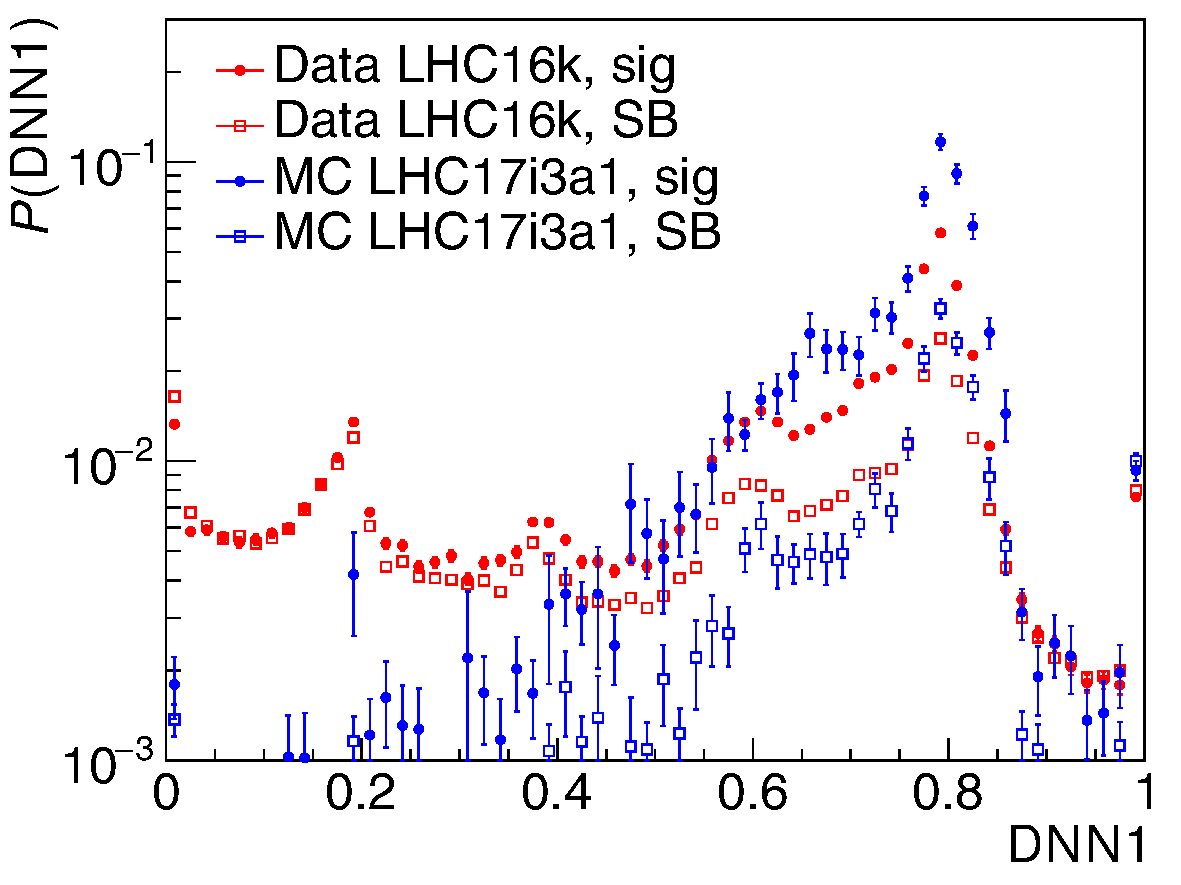
\includegraphics[width=0.5\textwidth]{eta_dnn_08_12_sb}}
%\caption{The $\lambda_0^2$ shower shape and DNN activation for the $\eta \rightarrow %\gamma\gamma$ signal and side-band region, comparing LHC16k with LHC17i3a1 MC.}
%\label{fig:eta_sb}
%\end{figure}

%In Fig.~\ref{fig:eta_lambda02}, the data/MC comparison is shown for the $\lambdasquare$ variable, where due to the weak shape dependence on single vs.\ two photons, the evolution from split to merged clusters is gradual.

%In Fig.~\ref{fig:eta_dnn}, the data/MC comparison is shown for the single photon DNN activation. A slight disagreement is visible at $0.8 < \mathrm{DNN1} < 0.9$, where the upper edge of the single photon peak falls slightly more steeply in data than in the MC. There is also slight disagreement between 0.26 and 0.3 in the $\lambdasquare$ variable for the same photon energy range, but it appears to be somewhat less pronounced.

%In Fig.~\ref{fig:eta_sb}, the data/MC comparison is shown for the $\lambdasquare$ and DNN variables separated for signal and side-band region. Since the MC does not reproduce all the physics processes in the data, the disagreement without side-band subtraction is expected.

%Some disagreement can be expected to arise due to the cross talk, which bleeds a small amount of the signal into neighboring electronics channels. However, we 
%bvj can unequivocally conclude 
%are convinced that the signal modeled by the MC is truly a single photon peak. Aside from this small bump, the region towards lower DNN1 is faithfully reproduced by MC.
%bvj , across 2 orders of magnitude. 
%This lends confidence that the region populated by both signal and background, where the template fitting is sensitive to the signal shape, is not affected by MC mismodelling. With increased $E_\gamma$, behavior analogous to $\pi^0 \rightarrow \gamma\gamma$ at lower $E_\gamma$ can be seen, where the diphoton clusters become merged.

%\subsection{Correlations and images}
%Figure~\ref{CorrelationLambdaDNN} shows the correlation between $\lambdasquare$ and neural network output, DNN, for clusters with {14$<\pt<$15 \GeVc} in p-Pb data that pass the selection described in Section~\ref{sec:clusterselection} including the isolation cut.  

%The sharp peak in $\lambdasquare$ is strongly correlated with the peak at DNN$\approx 0.75$, and the tail/bump structure in $\lambdasquare$ is correlated with the peak at DNN$\approx 0.2$. This shows that if these variables were used for binary classification, suitable cuts on both variables would largely agree. For example, about 70$\%$ of the clusters with {$\lambdasquare<0.4$} also have {DNN$>0.55$}, whereas 80$\%$ of the clusters with DNN$>0.55$ also have {$\lambdasquare<0.4$}.

%\begin{figure}[h]
%\center
%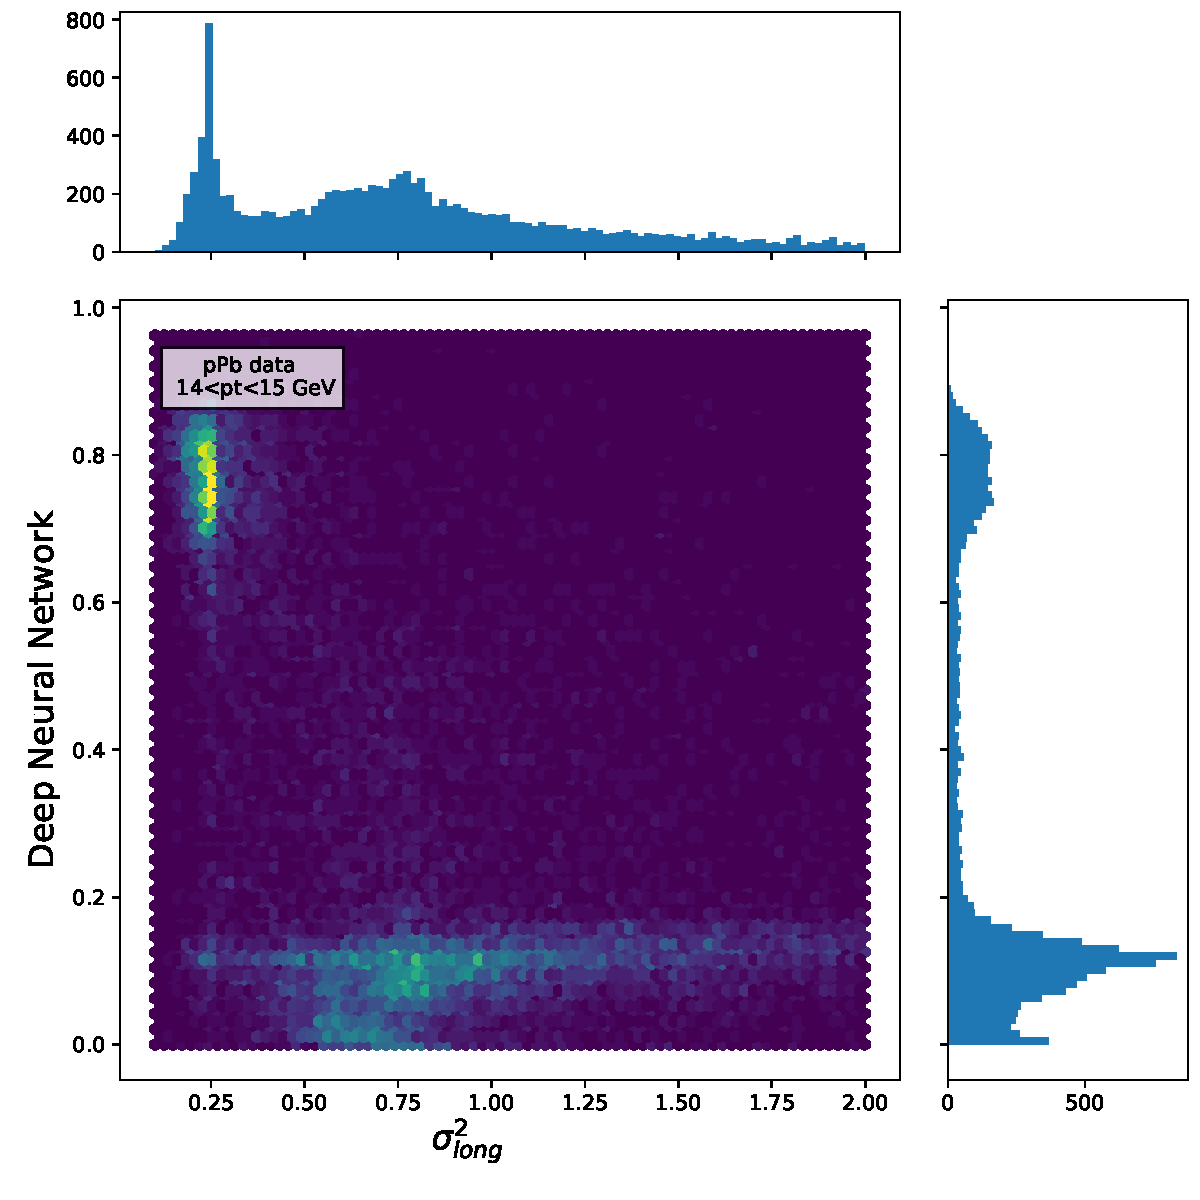
\includegraphics[width=0.495\textwidth]{PhotonID/Lambda_NN1_correlation}
%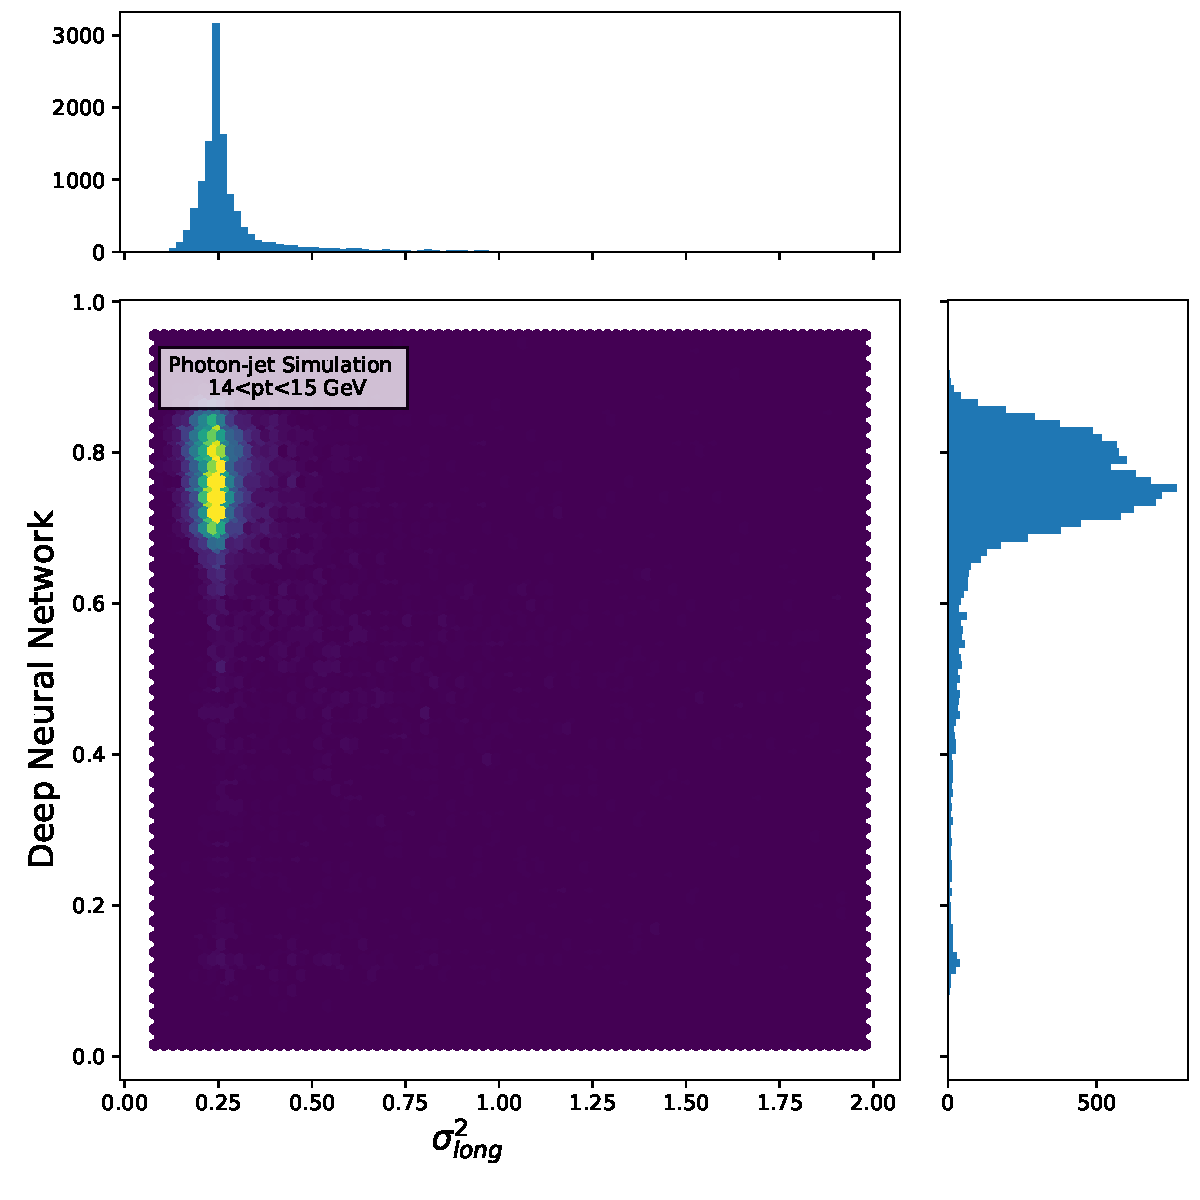
\includegraphics[width=0.495\textwidth]{PhotonID/Photon-jet_simulation_DNN_lambda}
%\caption{Correlation between $\lambdasquare$ variable and neural network for clusters within the range {14--15 \GeVc} in p-Pb data (left) and photon+jet simulation (right). The color code range is truncated for better visibility of the features of the data.}
%\label{CorrelationLambdaDNN}
%\end{figure}

%However, in this analysis we do not use these shower-shape variables for binary classification. Instead, we perform a shape analysis to extract our purity with the template fit method, as shown in Section~\ref{sec:purity}. Therefore, the use of these two variables, which have very different distributions, is not redundant.

% Figure~\ref{CorrelationDNNE} shows the correlation between DNN and the ratio of the energy in the leading cell to the total cluster energy $\emax$, which represents a rudimentary shower-shape variable. The correlation shows that low values of neural network select mostly clusters with $\emax$ in the range around 0.5, which are likely the product of symmetric $\pi^{0}\to\gamma\gamma$ decays. On the other hand, the large values of neural-network output corresponds to clusters with large values of $\emax$. Quantitatively, about 70$\%$ of the clusters with {$\emax>0.7$} also have {DNN$>0.55$}, whereas 80$\%$ of the clusters with DNN$>0.55$ also have $\emax<0.3$.

% \begin{figure}[h]
% \center 
% \includegraphics[width=0.495\textwidth]
% {PhotonID/DNN_emax_over_e_correlation}
% 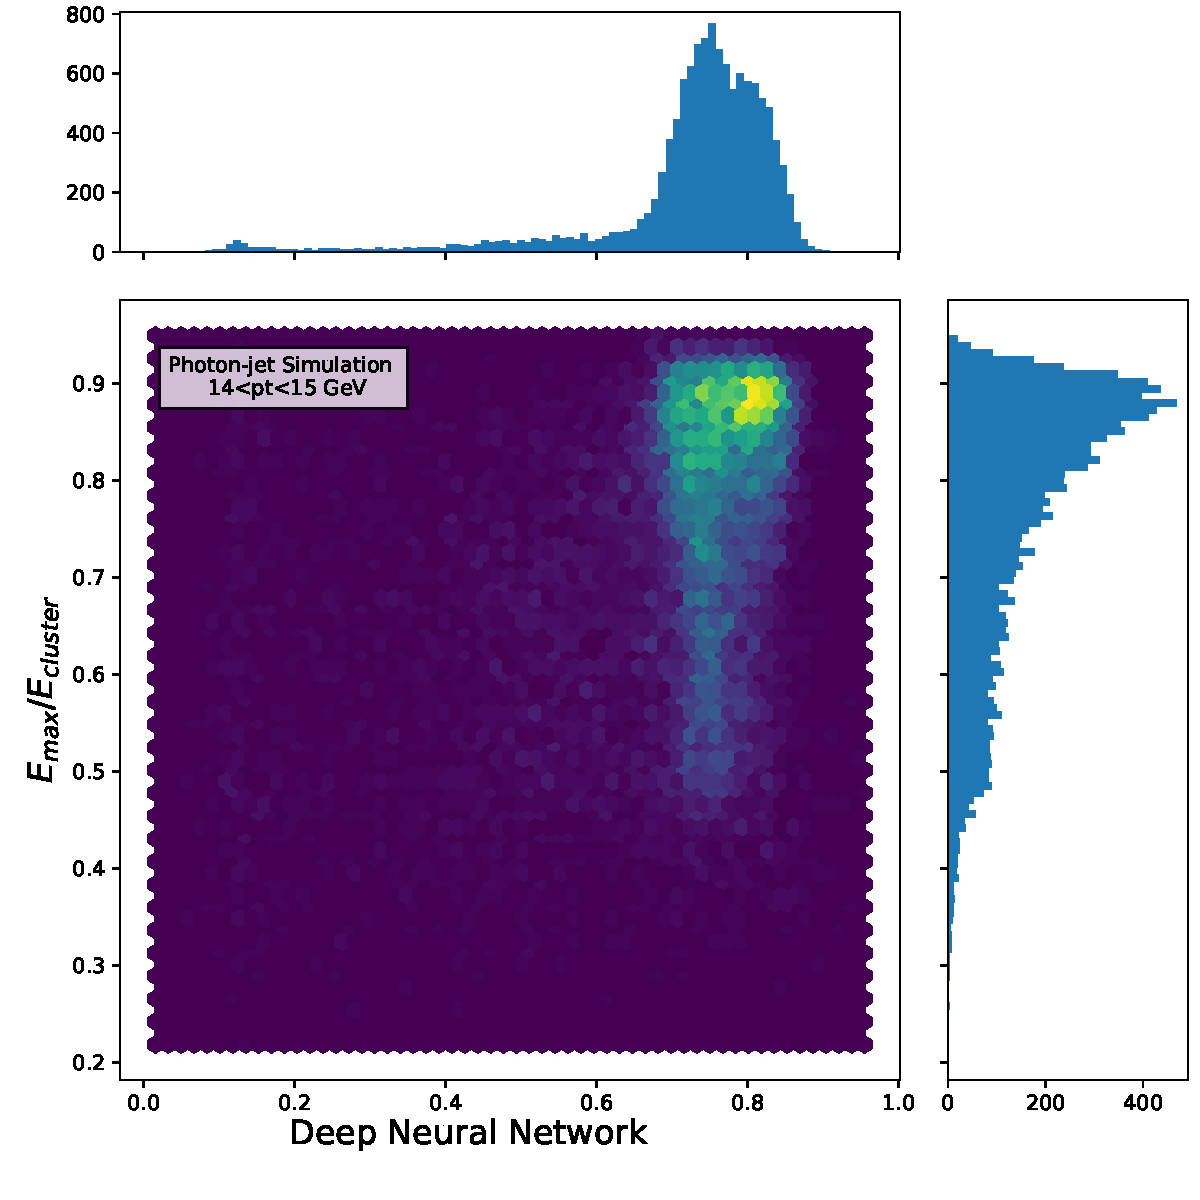
\includegraphics[width=0.495\textwidth]{PhotonID/Photon-jet_simulation_emax_over_ecluster_DNN}
% \caption{Correlation between $\emax$ variable and neural network output for clusters within the range {14--15 \GeVc} in p-Pb data (left) and photon+jet simulation (right).}
% \label{CorrelationDNNE}
% \end{figure}

%Figure~\ref{ClusterImages} shows a random selection of cluster shower shapes for clusters with {12$<\pt<$16 \GeVc} in pp data. The shower shapes are sorted by their DNN score, but the corresponding $\lambdasquare$ value is also shown for comparison. The clusters with DNN$>0.55$ are labeled as green, whereas the ones with DNN$<0.3$ are labeled with red. The clusters with DNN$>0.55$ deposit most of their energy (around 80$\%$ or more) in a single cell in most cases; this is the expected shower shape for photons as the cell dimensions are designed to be similar to the Moliere radius. On the other hand, the clusters with DNN$<0.3$ selection are much larger, have a more irregular shape, and often contain two maxima with similar strength, which is what we expect from $\pi^{0}$ decays that yield two showers that are not fully merged in a single cell.

%\begin{sidewaysfigure}
%\center
%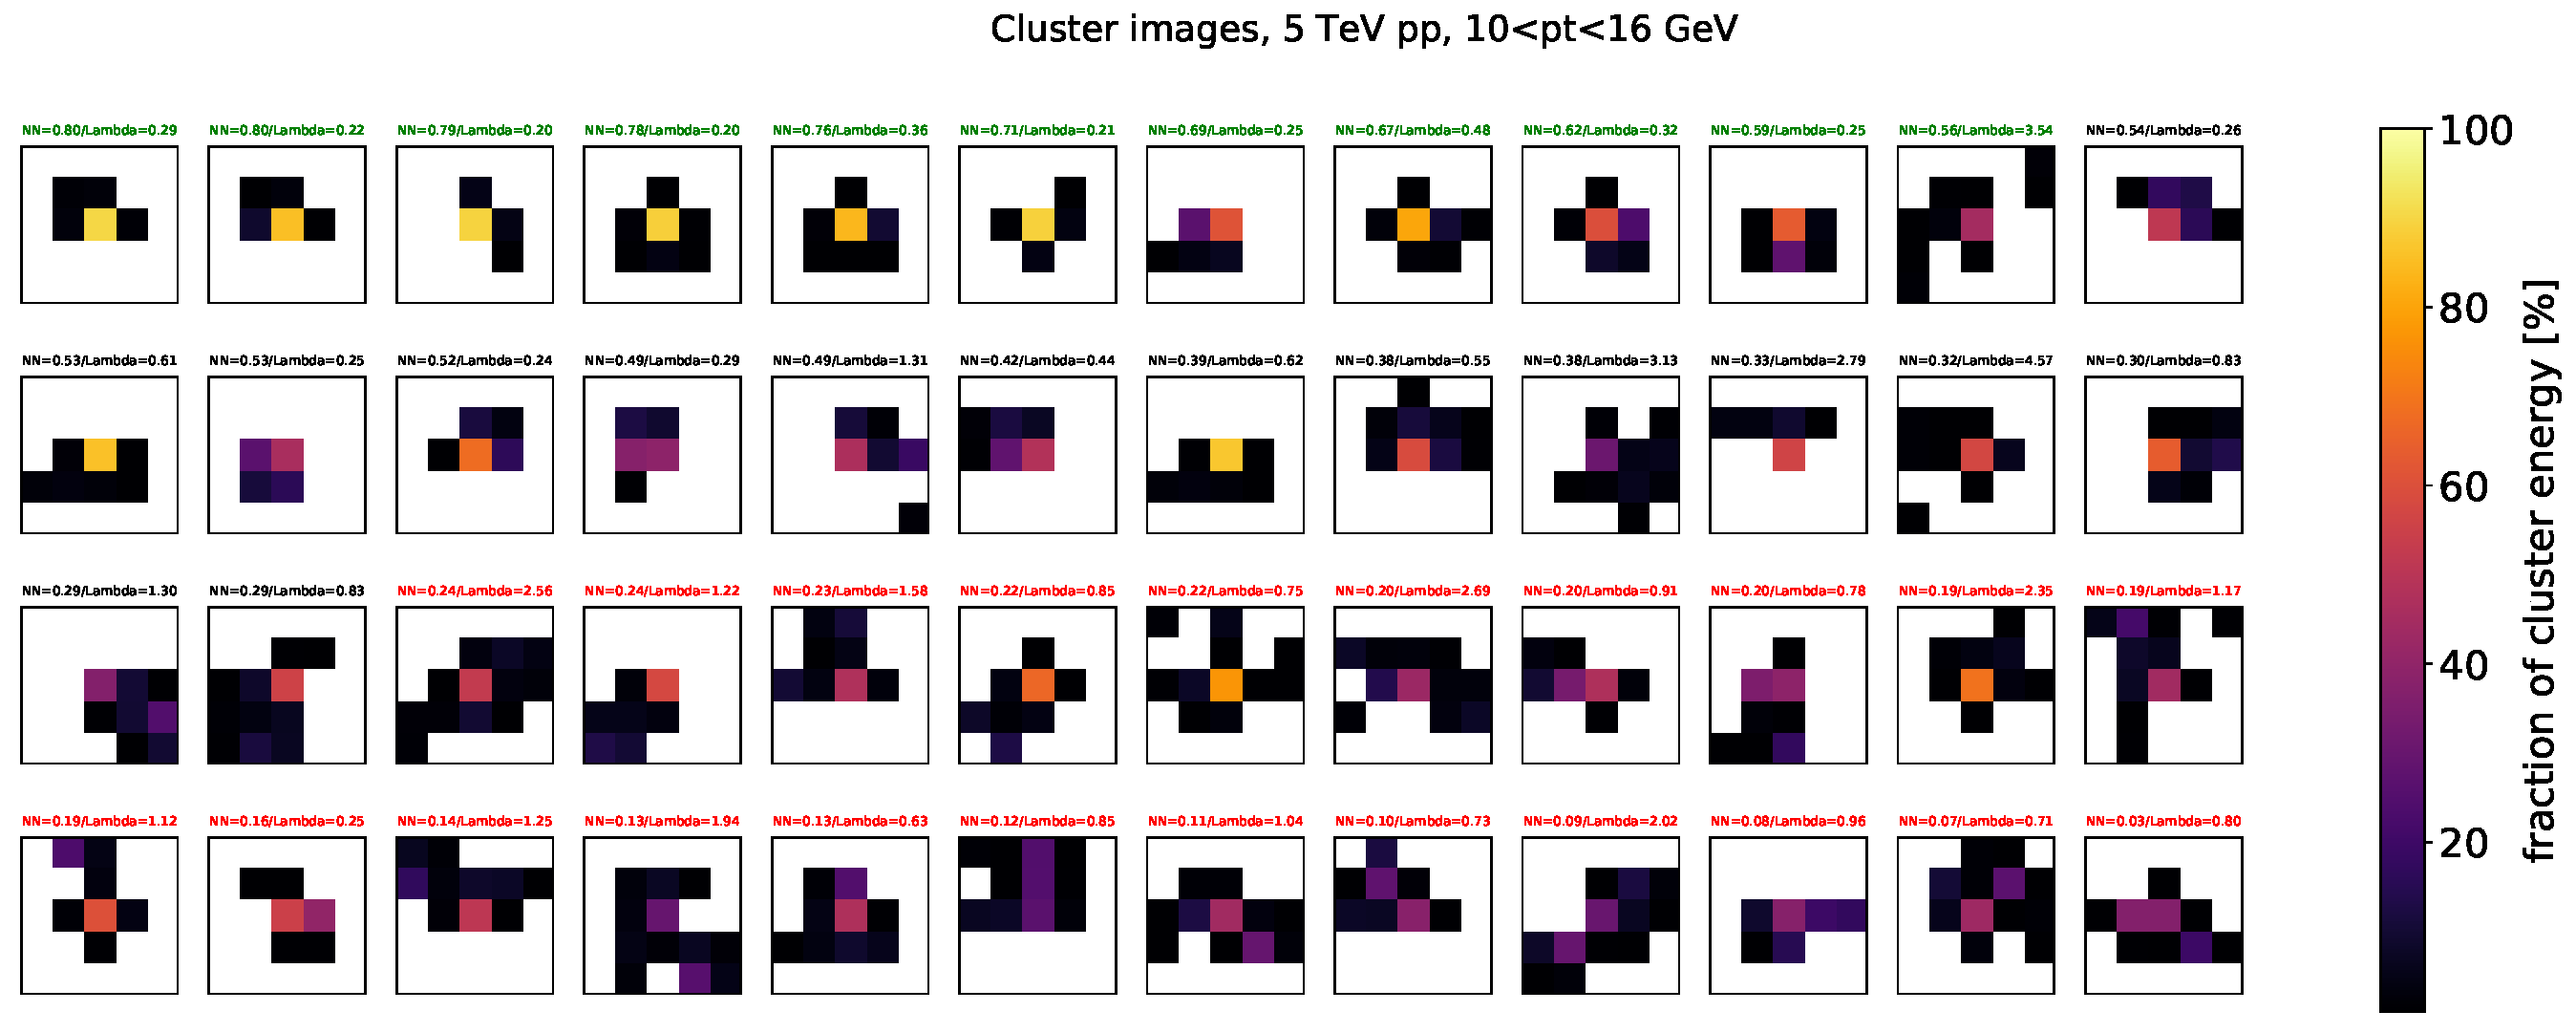
\includegraphics[width=1.0\textwidth]{PhotonID/ClusterImagesExample}
%\caption{Random selection of cluster shower-shape images of pp 5 TeV data for clusters that pass our selection. The color code represents the fraction of the total cluster energy that is within a given cell. Only cells around a matrix of 5$\times$5 cells around the seed cell of the cluster are shown. The images are sorted according to the output of the neural network from the upper left to the bottom right; the corresponding $\lambdasquare$ variable is also shown for each image. The title of the images passing our photon selection are shown in green, whereas the ones of the images passing our $\pi^{0}$ selection are shown in red.}
%\label{ClusterImages}
%\end{sidewaysfigure}
